\documentclass[12pt,a4paper]{article}
\usepackage[T1]{fontenc}
\usepackage{ae,aecompl}
\usepackage{color}	% Farbunterstützung
\usepackage{amssymb}	% Mathe
\usepackage{amsmath} % Mathe
\usepackage[utf8]{inputenc} % Direkte Eingabe von Umlauten und anderen Diakritika
\usepackage{graphicx}
%\renewcommand{\rmdefault}{\sfdefault} 
%\renewcommand{\baselinestretch}{1.5}         
\usepackage{fullpage}
\usepackage{apacite}

\author{Norman Lemke, Moritz Süß}

\begin{document}
  \title{Session II: Introduction to Human Capital}
  \maketitle
  \tableofcontents
  \thispagestyle{empty}
  \pagebreak


  \part{Meeting 2} % (fold)
  \label{prt:Meeting 2}
  \section{Questions} % (fold)
  \begin{itemize}
    \item Becker
      \begin{itemize}
        \item What is human capital, what kinds of human capital are discussed
          \begin{itemize}
            \item training, education, health, morale, etc.
          \end{itemize}
        \item What is the basic model (NPV etc., see below)
        \item Go through the stylized facts \& find the answers given by Becker (see below)
      \end{itemize}
    \item Ben-Porath
	  \begin{itemize}
	    \item Does the model portray a realistic view of the labour market? \\
	      \emph{Challenge of discerning between time spent educating and working. Possibility of doing both at same time. Possibility of being paid for work experience not educational, unpaid study time.}
	    \item How does this model, if significant and supported by evidence, help policy makers? \\
	      Difficulty of measuring $s_t$. Rate of interest $r$, the rental price of human capital $a_0$ and price of purchased inputs $P_d$ can be influenced.
	    \item In which case could $\delta$ (the rate of deterioration) be negative?
	  \end{itemize}
    
	\item Lazear
	  \begin{itemize}
	    \item How does the skill-weights view alleviate some of the problems of classical firm-specific human capital? \\
	      \emph{Firm-specific human capital seems difficult to prove, since most knowledge is at least somewhat universal. An approach based on the relative knowledge of general skills is more applicable/realistic.}
	    \item (page 17) What are possible drawbacks of this approach? \\
	      \emph{Jobs may not pay for skills beyond a certain point (overqualification) or may exhibit diminishing returns on skills. Does not take into account not getting a job at all because of lower bound on skills. Relative skill requirements mean it could be a optimal strategy to train one skill more than would be required in absolute terms since the other skill was trained too much in relative terms.}

	  \end{itemize}
	

  \end{itemize}
  % part Questions (end)
  \section{Becker} % (fold)
  \label{prt:Becker}

  % part Becker (end)
  \subsection{Stylized Facts} % (fold)
  \begin{enumerate}
    \item Earnings typically increase with age at a decreasing rate. Both the rate of increase and the rate of retardation tend to be positively related the level of skill.\\
      \begin{figure}[ht]
        \centering
        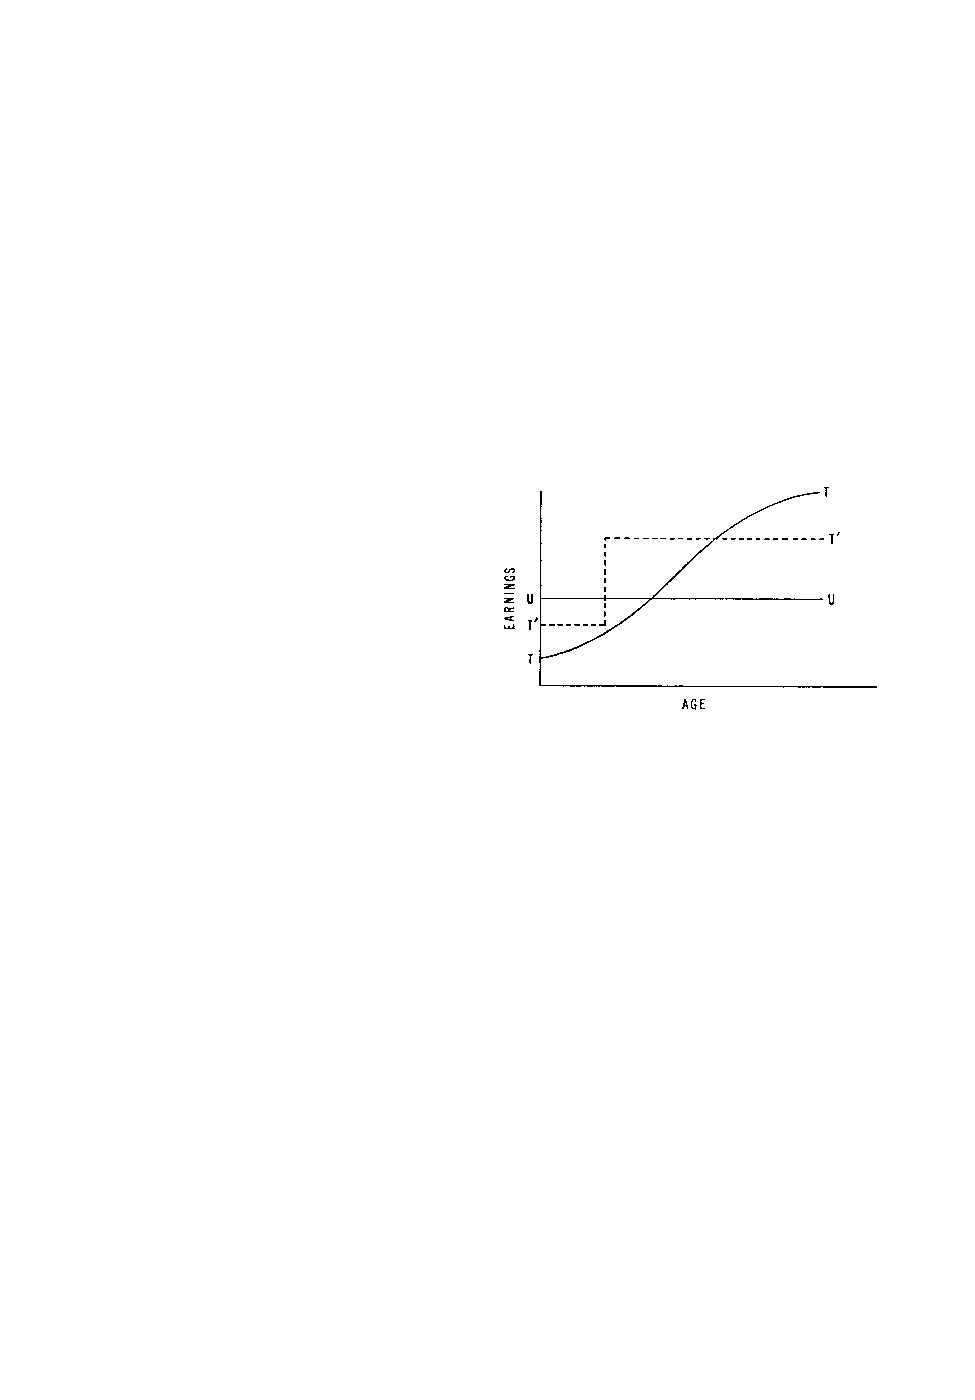
\includegraphics[width=8cm]{fig1.pdf}
        \caption{from Becker, p.15}
        \label{fig1}
      \end{figure}
      UU is the untrained person, TT trained person (first paying for, then collecting rent from training). Difference between UU and TT greater the greater the cost of and return from training. Not only does training make the curve steeper, but also more concave. Extreme case TT'.
    \item Unemployment rates tend to be negatively related to the level of skill
      \begin{itemize}
        \item market demand, $MP$...
      \end{itemize}
    \item Firms in underdeveloped countries appear to be more
      "paternalistic" toward employees than those in developed countries
      \begin{itemize}
        \item investment in activities outside the job are done when an
          increase in productivity is the result
        \item e.g. health, anti-alcoholism
        \item thus, this "paternalistic" behavior results from typical
          behavior outside the firm!
      \end{itemize}
    \item Younger persons change jobs more frequently and receive more
      on-the-job training than older persons
      \begin{itemize}
        \item decisions regarding human capital are NPV decisions
        \item therefore, they are driven by the time-frame of the
          decision (on-the-job training)
      \end{itemize}
    \item The distribution of earnings is positively skewed, especially
      among professional and other skilled workers
    \item Abler persons receive more education and other kinds of
      training than others
      \begin{itemize}
        \item higher $MP$...
      \end{itemize}
    \item The division of labour is limited by the extent of the
      market
      \begin{itemize}
        \item a larger market generates \emph{incentives} for more
          specialization, as higher investments in education are
          rewarded by higher wages
        \item thus, a "larger market" implies more demand for
          specialized skills...
      \end{itemize}
    \item the typical investor in human capital is more impetuous and thus
      more likely to err than is the typical investor in tangible capital
  \end{enumerate}
  % section stylized facts (end)

  \subsection{Basic Model} % (fold)
  \label{sec:model}
  \begin{eqnarray}
    MP &=& w
  \end{eqnarray}
  Workers have different unique productivities (wages) in each period.
  \begin{eqnarray}
    MP_{t}&=&w_{t}
  \end{eqnarray}
  Training lowers current receipts (R) and raises current expenditures
  (E). However this trend is reversed for future periods. Therefore: NPV
  consideration.
  \begin{eqnarray}
    \sum_{t=0}^{n-1} \dfrac{R_t}{(1+i)^{t+1}} &=& \sum_{t=0}^{n-1}
    \dfrac{E_t}{(1+i)^{t+1}}
  \end{eqnarray}
  Now we only have training in the first period; Expenditures in first
  period are wages + cost of training (k); afterwards only wage. Receipts
  in all periods is MP.
  \begin{eqnarray}
    MP_0 + \sum_{t=0}^{n-1} \dfrac{MP_t}{(1+i)^{t}} &=& W_0 + k +
    \sum_{t=0}^{n-1} \dfrac{W_t}{(1+i)^{t}} \label{eq4}
  \end{eqnarray}
  We define term $G$
  \begin{eqnarray}
    G&=& \sum_{t=1}^{n-1} \dfrac{MP_t - W_t}{(1+i)^{t}}
  \end{eqnarray}
  Now equation (\ref{eq4}) becomes
  \begin{eqnarray}
    MP_0 + G &=& W_0 + k \label{eq6}
  \end{eqnarray}
  Now we need to include the fact that training takes away time from
  production. ($MP'_0$ what could have been produced, $MP_=$ what was
  actually produced, C is the sum of opportunity cost and the outlays on
  training) Equation (\ref{eq6}) becomes
  \begin{eqnarray}
    MP'_0 + G &=& W_0 + C \label{eq7}
  \end{eqnarray}
  We see that G is the excess of future receipts over future outlays (a
  notion of return on training). Optimality condition: $G=C$ (return
  equals cost)
  % section model (end)

  \subsubsection{General Training} % (fold)
  \label{sub:general_training}
  \textbf{General Training:} This kind of training generally increases
  the $MP$ of the worker. Since the worker can switch jobs, he will
  have to bear the costs of this kind of training.

  Hence, $MP$ and $W$ are raised by the same amount! $MP_t = W_t
  \forall t$ 
  \begin{eqnarray}
    G&=& \sum_{t=1}^{n-1} \dfrac{MP_t - W_t}{(1+i)^{t}}=0
  \end{eqnarray}
  Thus, eq. (\ref{eq7}) becomes 
  \begin{eqnarray}
    MP'_0 &=& W_0 +C \\
    \rightarrow W_0 &=& MP'_0 -C
  \end{eqnarray}
  % subsection General Training (end)
  \subsubsection{Specific Training} % (fold)
  \label{sub:Specific_Training}
  \textbf{Specific Training:} This kind of training only increases the
  $MP$ of the worker for the specific firm.
  Consequently, in this extreme case firms are willing to pay for the
  training, since the investment is offset by increases in profit due
  to higher $MP$ of the workers. On the other hand, workers will not
  be willing to invest, since they have "no gain" from this kind of
  investment. The gain is fully absorbed by the firm!
  % subsubsection Specific Training (end)

  \section{Ben-Porath} % (fold)
  \subsection{Fact sheet} % (fold)
  \begin{enumerate}
    \item People make most of their investments in themselves when they are young, and to a large extend by foregoing current earnings.
	\item The larger the stock of human capital, the larger the earnings per unit of time that the individual could get in the market and therefore the higher the foregone earnings from diverting a unit of time away from the market.
	\item If $\gamma _{1} = \gamma _{2}$ (Cobb-Douglas: Equation (17), p. 360) the more highly educated person is also better equipped for learning, so that his higher opportunity cost is matched by the greater amount of skills that he can acquire per hour.
	\item If $\gamma _{2} > \gamma _{1}$ capital accumulation reduces the cost of producing human capital, and it is possible even in phase (ii) to have a stretch of time over which investment rises.
	\item Three phases will exist:
	  \begin{itemize}
	    \item Available stock of human capital $K_t$ is not large enough to satisfy demand.
	    \item Available stock is enough to supply the services demanded, so that $0<s<1$ and the services of human capital are truly a variable factor.
	    \item Stock of capital is too big so that the optimal policy requires more disinvestment than is feasible through deterioration, that is to produce negative quantities of human capital.
	  \end{itemize}
	\item \emph{Normal case}: Capital stock does rise over a period, eventually as gross additions become very small and the stock becomes large this must be reversed, and toward end of life, $T$, the stock will decline, if there is any deterioration.
	\item $\dot{I}$ is always negative. Thus the curve of observed earnings exaggerates the rate of increase of earning capacity when the latter increases and understates its decline when it declines.
	\item If depreciation is zero, there is always, except at point $T$, an increase in the three types of earnings ($E_t$ - disposable earnings, $Y_t$ - earning capacity, $\hat{E}$ - observed earnings), and at each point in time their rank by rate of change will be the reverse of their rank by level.
	\item If there is no deterioration ($\delta = 0$) the ever rising curve of observed earnings is always concave from below.
	\item Possibility that optimal decision requires initial assignment of $s=1$, or $100\%$ of the labour force educating themselves.
  \end{enumerate}

  \section{Lazear} % (fold)
  \subsection{Fact sheet} % (fold)
  \begin{enumerate}
    \item The ``skill-weights" view allows skills to be general instead of firm-specific. Instead the relative importance of skills makes them more or less attractive to employers.
    \item $y_i = \lambda_i A+(1-\lambda_i)B$ is the potential earning for a worker with skill set $(A, B)$ at firm $i$.
    \item $\lambda_i$ reflects that firm $i$ may weigh the two skills differently.
    \item $p$ is the probability that the worker is going to stay with the current company in the next period.
    \item The difference between the earnings growth associated with a given amount of experience for those who stay and those who go leads on the \emph{tenure coefficient}. The amount of wage growth the leavers get loads on the experience coefficient.
    \item The worker must chose his investment strategy not knowing whether he will leave the firm or not. $p$ is usually large enough so that he caters to the needs of the first job. When he looses his job he will also loose some income since his skill set will most likely be poorly matched to the new job.
    \item The lower $p$, the less he looses through being let off.
    \item The tenure coefficient should be negatively related to the amount of turnover in the occupation.
    \item Those who leave a firm with unusual weighting patterns suffer larger wage loss for a given $p$.
    \item $Market thickness$ is modeled as allowing more search: Two draws occur, for the second of which the worker can decide whether to switch jobs or not.
    \item In thicker markets a worker looses less on a move despite a more idiosyncratic investment strategy.
	\item Investment increases over time because except for a perfect match between the preferences of the first and second company another round of investment is appropriate.
	\item Shown with data: It is possible to generate tenure coefficients that are nearly the same size as the experience coefficients ($90\%$).
	\item The higher $p$, the large the tenure coefficient.
	\item When $\lambda$ takes extreme values it tends to be far away from $\bar{\lambda}$, which is why the uniform distribution yields lower tenure coefficients than the bimodal.
  \end{enumerate}

\part{Meeting 4} % (fold)
\label{prt:Meeting 4}
\section{(Destré et al., 2006) "Learning form experience or learning from others?"} % (fold)
  \label{sec:Destré et al., 2006}
  
  % section Destré et al., 2006 (end)

\section{(Ertaut, 2000) "Non-formal learning and tacit knowledge in professional work"} % (fold)
 \label{sec:(Ertaut, 2000}
 
 % section (Ertaut, 2000 (end)
% part Meeting 4 (end)



  %\bibliographystyle{apacite} 
  %\bibliography{lit}
\end{document}
